\documentclass[11pt,a4paper]{article}

% Packages
\usepackage[utf8]{inputenc}
\usepackage[T1]{fontenc}
\usepackage{amsmath,amssymb,amsfonts}
\usepackage{graphicx}
\usepackage{tikz}
\usepackage{tikz-3dplot}
\usepackage{pgfplots}
\usepackage{xcolor}
\usepackage{geometry}
\usepackage{fancyhdr}
\usepackage{hyperref}
\usepackage{listings}
\usepackage{algorithm}
\usepackage{algpseudocode}
\usepackage{booktabs}
\usepackage{subcaption}
\usepackage{physics}

% TikZ libraries
\usetikzlibrary{arrows.meta,positioning,shapes.geometric,calc,patterns,decorations.pathmorphing,3d,angles,quotes}
\pgfplotsset{compat=1.18}

% Page setup
\geometry{margin=1in}
\pagestyle{fancy}
\fancyhf{}
\rhead{X-Band Radar Simulation}
\lhead{Technical Documentation}
\rfoot{Page \thepage}

% Colors
\definecolor{radargreen}{RGB}{0,255,0}
\definecolor{raycolor}{RGB}{255,165,0}
\definecolor{targetcolor}{RGB}{255,0,0}
\definecolor{groundcolor}{RGB}{139,90,43}
\definecolor{skycolor}{RGB}{135,206,235}
\definecolor{beamcolor}{RGB}{255,255,0}

% Code style
\lstset{
    basicstyle=\ttfamily\small,
    keywordstyle=\color{blue},
    commentstyle=\color{gray},
    numbers=left,
    numberstyle=\tiny\color{gray},
    frame=single,
    breaklines=true
}

\title{\textbf{X-Band Radar Simulation}\\
\Large Complete Technical Documentation\\[1em]
\normalsize From Ray Tracing to PPI Display}
\author{Radar Simulation Framework}
\date{\today}

\begin{document}

\maketitle
\tableofcontents
\newpage

%=============================================================================
\section{System Overview}
%=============================================================================

This document provides a complete technical description of the X-band radar simulation software, covering every stage from 3D world construction to final PPI display rendering.

\subsection{High-Level Pipeline}

\begin{figure}[htbp]
\centering
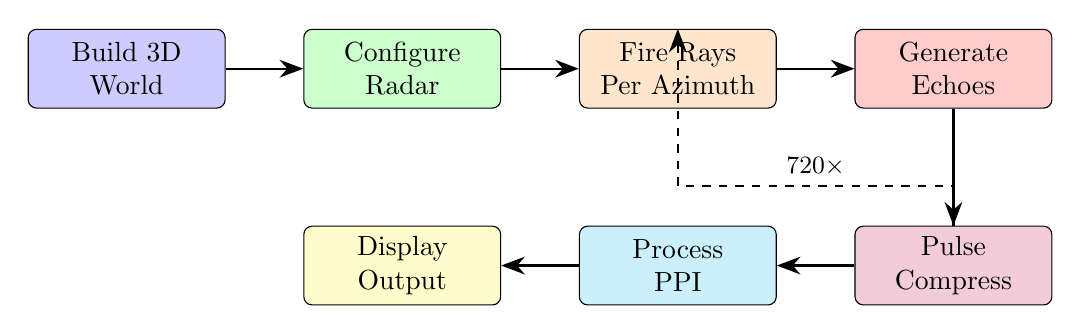
\begin{tikzpicture}[
    box/.style={rectangle, draw, minimum width=2.5cm, minimum height=1cm, align=center, rounded corners=3pt},
    arrow/.style={-{Stealth[length=3mm]}, thick}
]
    % Main pipeline boxes
    \node[box, fill=blue!20] (world) at (0,0) {Build 3D\\World};
    \node[box, fill=green!20] (config) at (3.5,0) {Configure\\Radar};
    \node[box, fill=orange!20] (rays) at (7,0) {Fire Rays\\Per Azimuth};
    \node[box, fill=red!20] (signal) at (10.5,0) {Generate\\Echoes};

    \node[box, fill=purple!20] (compress) at (10.5,-2.5) {Pulse\\Compress};
    \node[box, fill=cyan!20] (ppi) at (7,-2.5) {Process\\PPI};
    \node[box, fill=yellow!20] (display) at (3.5,-2.5) {Display\\Output};

    % Arrows
    \draw[arrow] (world) -- (config);
    \draw[arrow] (config) -- (rays);
    \draw[arrow] (rays) -- (signal);
    \draw[arrow] (signal) -- (compress);
    \draw[arrow] (compress) -- (ppi);
    \draw[arrow] (ppi) -- (display);

    % Loop indication
    \draw[arrow, dashed] (compress.north) -- ++(0,0.5) -| node[above, pos=0.25] {\small 720$\times$} (rays.north);

\end{tikzpicture}
\caption{High-level simulation pipeline. The ray-to-compress loop executes 720 times (once per azimuth).}
\label{fig:pipeline}
\end{figure}

\subsection{Key Parameters}

\begin{table}[htbp]
\centering
\begin{tabular}{lll}
\toprule
\textbf{Parameter} & \textbf{Value} & \textbf{Derived From} \\
\midrule
Center Frequency & $f_0 = 9.41$ GHz & X-band marine radar \\
Wavelength & $\lambda = 3.19$ cm & $\lambda = c/f_0$ \\
Bandwidth & $B = 50$ MHz & Chirp sweep \\
Pulse Width & $T = 10$ $\mu$s & Waveform design \\
Range Resolution & $\Delta R = 3.0$ m & $\Delta R = c/(2B)$ \\
Beamwidth (H) & $\theta_{3dB} = 3.9°$ & Antenna aperture \\
Azimuths & 720 & 0.5° spacing \\
Rays per Azimuth & 2000 & Monte Carlo sampling \\
\bottomrule
\end{tabular}
\caption{Primary simulation parameters}
\label{tab:params}
\end{table}

%=============================================================================
\section{Stage 1: 3D World Construction}
%=============================================================================

\subsection{Scene Geometry}

The simulation world is constructed from triangle meshes. Each target is defined by vertices and faces, positioned at specific coordinates.

\begin{figure}[htbp]
\centering
\tdplotsetmaincoords{70}{110}
\begin{tikzpicture}[tdplot_main_coords, scale=0.8]
    % Ground plane
    \fill[groundcolor!30] (-6,-6,0) -- (6,-6,0) -- (6,6,0) -- (-6,6,0) -- cycle;
    \draw[groundcolor, thick] (-6,-6,0) -- (6,-6,0) -- (6,6,0) -- (-6,6,0) -- cycle;
    \draw[groundcolor!50, thin] (-6,0,0) -- (6,0,0);
    \draw[groundcolor!50, thin] (0,-6,0) -- (0,6,0);

    % Radar at origin
    \shade[ball color=green!70] (0,0,0.3) circle (0.3);
    \node[below] at (0,0,0) {\small Radar};

    % Target 1: Corner reflector NE (at 45°, 4 units = 200m scaled)
    \begin{scope}[shift={(2.83,2.83,0)}]
        \fill[targetcolor!70] (0,0,0) -- (1,0,0) -- (0,1,0) -- cycle;
        \fill[targetcolor!50] (0,0,0) -- (0,1,0) -- (0,0,1) -- cycle;
        \fill[targetcolor!90] (0,0,0) -- (1,0,0) -- (0,0,1) -- cycle;
        \node[above right] at (0.5,0.5,0.5) {\small Target 1};
    \end{scope}

    % Target 2: Sphere W (at 270°, 2 units = 100m scaled)
    \begin{scope}[shift={(-2,0,0.5)}]
        \shade[ball color=blue!50] (0,0,0) circle (0.4);
        \node[left] at (-0.5,0,0) {\small Target 2};
    \end{scope}

    % Target 3: Corner S (at 180°, 6 units = 300m scaled)
    \begin{scope}[shift={(0,-6,0)}]
        \fill[targetcolor!60] (0,0,0) -- (0.8,0,0) -- (0,0.8,0) -- cycle;
        \fill[targetcolor!40] (0,0,0) -- (0,0.8,0) -- (0,0,0.8) -- cycle;
        \node[below] at (0,-0.3,0) {\small Target 3};
    \end{scope}

    % Coordinate axes
    \draw[-{Stealth}, thick] (0,0,0) -- (2,0,0) node[right] {$x$ (E)};
    \draw[-{Stealth}, thick] (0,0,0) -- (0,2,0) node[above] {$y$ (N)};
    \draw[-{Stealth}, thick] (0,0,0) -- (0,0,2) node[above] {$z$};

    % Range rings (projected)
    \draw[dashed, gray] (0,0,0) circle (2);
    \draw[dashed, gray] (0,0,0) circle (4);
    \node[gray] at (2.2,0.3,0) {\tiny 100m};
    \node[gray] at (4.2,0.3,0) {\tiny 200m};

\end{tikzpicture}
\caption{3D scene with radar at origin and multiple targets. Ground plane shown in brown. Range rings indicate distance from radar.}
\label{fig:scene3d}
\end{figure}

\subsection{Triangle Mesh Representation}

Every 3D object is decomposed into triangles:

\begin{figure}[htbp]
\centering
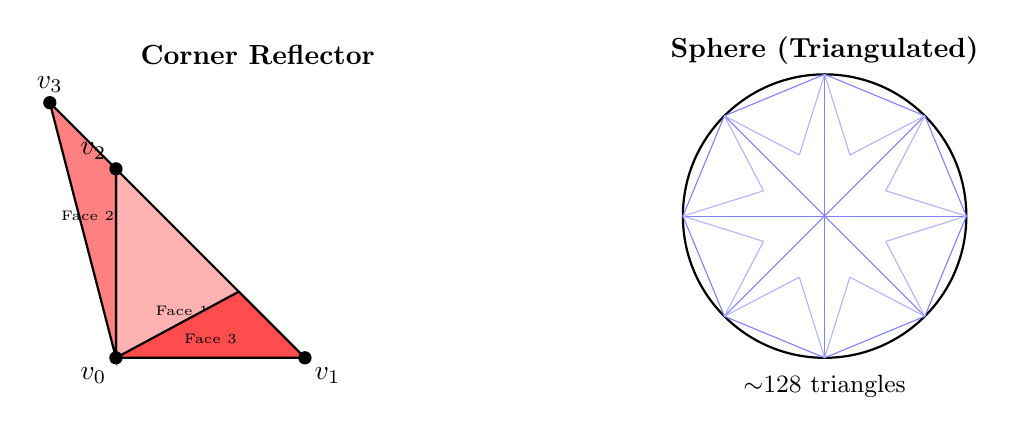
\begin{tikzpicture}[scale=1.2]
    % Corner reflector triangles
    \begin{scope}[shift={(0,0)}]
        \node[above] at (1.5,3) {\textbf{Corner Reflector}};

        % XY plane
        \fill[red!30] (0,0) -- (2,0) -- (0,2) -- cycle;
        \draw[thick] (0,0) -- (2,0) -- (0,2) -- cycle;
        \node at (0.7,0.5) {\tiny Face 1};

        % YZ plane (projected)
        \fill[red!50] (0,0) -- (0,2) -- (-0.7,2.7) -- cycle;
        \draw[thick] (0,0) -- (0,2) -- (-0.7,2.7) -- cycle;
        \node at (-0.3,1.5) {\tiny Face 2};

        % XZ plane (projected)
        \fill[red!70] (0,0) -- (2,0) -- (1.3,0.7) -- cycle;
        \draw[thick] (0,0) -- (2,0) -- (1.3,0.7) -- cycle;
        \node at (1,0.2) {\tiny Face 3};

        % Vertex labels
        \fill (0,0) circle (2pt) node[below left] {$v_0$};
        \fill (2,0) circle (2pt) node[below right] {$v_1$};
        \fill (0,2) circle (2pt) node[above left] {$v_2$};
        \fill (-0.7,2.7) circle (2pt) node[above] {$v_3$};
    \end{scope}

    % Sphere approximation
    \begin{scope}[shift={(6,0)}]
        \node[above] at (1.5,3) {\textbf{Sphere (Triangulated)}};

        % Draw icosphere-like mesh
        \draw[thick] (1.5,1.5) circle (1.5);

        % Triangle subdivisions
        \foreach \a in {0,45,...,315} {
            \draw[thin, blue!50] (1.5,1.5) -- ({1.5+1.5*cos(\a)},{1.5+1.5*sin(\a)});
        }
        \foreach \a in {0,45,...,315} {
            \draw[thin, blue!50] ({1.5+1.5*cos(\a)},{1.5+1.5*sin(\a)}) -- ({1.5+1.5*cos(\a+45)},{1.5+1.5*sin(\a+45)});
        }

        % Inner ring
        \foreach \a in {22.5,67.5,...,337.5} {
            \draw[thin, blue!30] ({1.5+0.7*cos(\a)},{1.5+0.7*sin(\a)}) -- ({1.5+1.5*cos(\a-22.5)},{1.5+1.5*sin(\a-22.5)});
            \draw[thin, blue!30] ({1.5+0.7*cos(\a)},{1.5+0.7*sin(\a)}) -- ({1.5+1.5*cos(\a+22.5)},{1.5+1.5*sin(\a+22.5)});
        }

        \node at (1.5,-0.3) {\small $\sim$128 triangles};
    \end{scope}
\end{tikzpicture}
\caption{Objects represented as triangle meshes. Left: Corner reflector (3 triangles). Right: Sphere approximated by icosphere subdivision.}
\label{fig:meshes}
\end{figure}

%=============================================================================
\section{Stage 2: Radar Configuration}
%=============================================================================

\subsection{Frequency and Wavelength}

The radar operates at X-band:

\begin{equation}
\lambda = \frac{c}{f_0} = \frac{2.998 \times 10^8 \text{ m/s}}{9.41 \times 10^9 \text{ Hz}} = 0.0319 \text{ m} = 3.19 \text{ cm}
\end{equation}

\subsection{Antenna Pattern}

The antenna gain pattern follows a sinc-squared approximation:

\begin{equation}
G(\theta) = G_0 \left[ \frac{\sin(\pi u)}{\pi u} \right]^2, \quad u = \frac{2.783 \cdot \theta}{\theta_{3dB}}
\end{equation}

\begin{figure}[htbp]
\centering
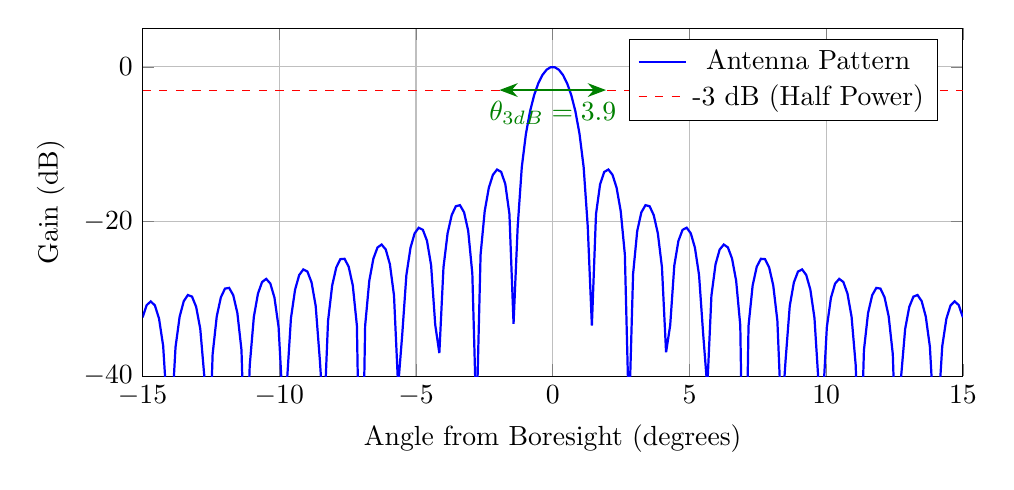
\begin{tikzpicture}
\begin{axis}[
    width=12cm, height=6cm,
    xlabel={Angle from Boresight (degrees)},
    ylabel={Gain (dB)},
    xmin=-15, xmax=15,
    ymin=-40, ymax=5,
    grid=both,
    legend pos=north east
]
    % Main lobe and sidelobes
    \addplot[thick, blue, domain=-15:15, samples=200] {
        20*log10(abs(sin(deg(pi*2.783*x/3.9))/(pi*2.783*x/3.9 + 0.0001)) + 0.0001)
    };
    \addlegendentry{Antenna Pattern}

    % 3dB line
    \addplot[dashed, red] coordinates {(-15,-3) (15,-3)};
    \addlegendentry{-3 dB (Half Power)}

    % Beamwidth annotation
    \draw[{Stealth}-{Stealth}, thick, green!50!black] (axis cs:-1.95,-3) -- (axis cs:1.95,-3);
    \node[green!50!black] at (axis cs:0,-6) {$\theta_{3dB} = 3.9°$};
\end{axis}
\end{tikzpicture}
\caption{Antenna gain pattern showing main lobe and sidelobes. The 3 dB beamwidth defines angular resolution.}
\label{fig:antenna_pattern}
\end{figure}

\subsection{Two-Way Pattern}

For monostatic radar (same antenna for TX and RX), the two-way pattern is:

\begin{equation}
G_{2-way}(\theta_{az}, \theta_{el}) = \left[ G(\theta_{az}) \cdot G(\theta_{el}) \right]^2
\end{equation}

This fourth-power relationship means the effective beamwidth is narrower than the one-way pattern.

%=============================================================================
\section{Stage 3: Ray Tracing}
%=============================================================================

\subsection{Ray Generation}

For each azimuth pointing direction, we generate 2000 rays distributed within the antenna beam:

\begin{figure}[htbp]
\centering
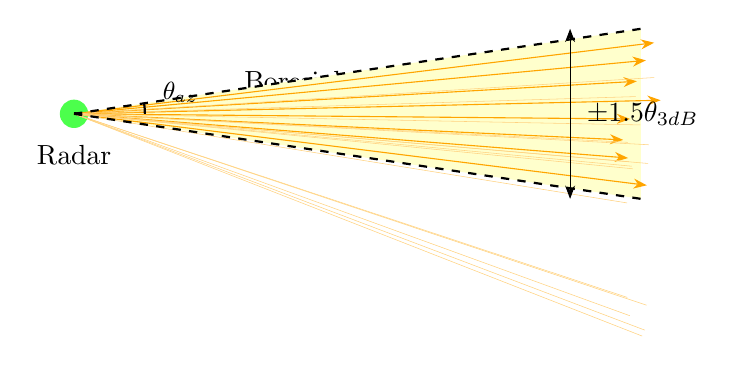
\begin{tikzpicture}[scale=0.9]
    % Radar
    \fill[green!70] (0,0) circle (0.2);
    \node[below] at (0,-0.3) {Radar};

    % Boresight direction
    \draw[-{Stealth}, very thick, black] (0,0) -- (8,0);
    \node[above] at (4,0.1) {Boresight ($\phi = 45°$)};

    % Beam cone (filled)
    \fill[beamcolor!20] (0,0) -- (8,1.2) -- (8,-1.2) -- cycle;

    % Individual rays
    \foreach \y in {-1.0,-0.7,-0.4,-0.1,0.2,0.5,0.8,1.1} {
        \pgfmathsetmacro{\randx}{0.3*rand}
        \draw[raycolor, thin, -{Stealth}] (0,0) -- ({8+\randx},{\y + 0.1*rand});
    }

    % More rays (denser)
    \foreach \i in {1,...,15} {
        \pgfmathsetmacro{\y}{-1.1 + 2.2*rand}
        \pgfmathsetmacro{\randx}{0.2*rand}
        \draw[raycolor!50, very thin] (0,0) -- ({8+\randx},{\y});
    }

    % Beam edges
    \draw[dashed, thick] (0,0) -- (8,1.2);
    \draw[dashed, thick] (0,0) -- (8,-1.2);

    % Beamwidth annotation
    \draw[{Stealth}-{Stealth}] (7,1.2) -- (7,-1.2);
    \node[right] at (7.1,0) {$\pm 1.5 \theta_{3dB}$};

    % Angle arc
    \draw[thick] (1,0) arc (0:8:1);
    \node at (1.5,0.3) {\small $\theta_{az}$};

\end{tikzpicture}
\caption{Ray generation for a single azimuth. 2000 rays are distributed randomly within $\pm 1.5 \times$ beamwidth of boresight. Orange arrows show individual rays.}
\label{fig:ray_generation}
\end{figure}

\subsection{Ray Direction Calculation}

Each ray direction is computed from azimuth and elevation offsets:

\begin{align}
\phi_{ray} &= \phi_{boresight} + \Delta\phi, \quad \Delta\phi \sim \mathcal{U}(-1.5\theta_{az}, +1.5\theta_{az}) \\
\theta_{ray} &= \Delta\theta, \quad \Delta\theta \sim \mathcal{U}(-1.5\theta_{el}, +1.5\theta_{el})
\end{align}

The unit direction vector is:
\begin{equation}
\hat{d} = \begin{pmatrix}
\cos(\theta_{ray}) \cos(\phi_{ray}) \\
\cos(\theta_{ray}) \sin(\phi_{ray}) \\
\sin(\theta_{ray})
\end{pmatrix}
\end{equation}

\subsection{Ray-Triangle Intersection}

We use the Möller-Trumbore algorithm to find where each ray intersects scene triangles.

\begin{figure}[htbp]
\centering
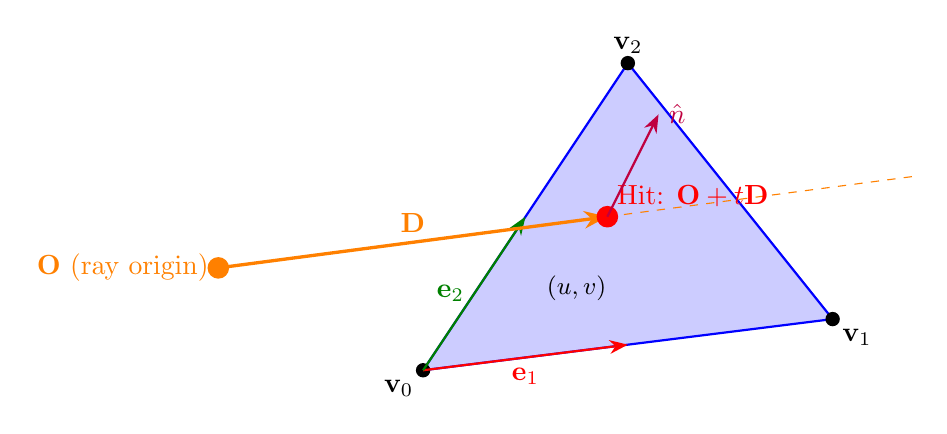
\begin{tikzpicture}[scale=1.3]
    % Triangle
    \coordinate (v0) at (0,0);
    \coordinate (v1) at (4,0.5);
    \coordinate (v2) at (2,3);

    \fill[blue!20] (v0) -- (v1) -- (v2) -- cycle;
    \draw[thick, blue] (v0) -- (v1) -- (v2) -- cycle;

    % Vertex labels
    \fill (v0) circle (2pt) node[below left] {$\mathbf{v}_0$};
    \fill (v1) circle (2pt) node[below right] {$\mathbf{v}_1$};
    \fill (v2) circle (2pt) node[above] {$\mathbf{v}_2$};

    % Edge vectors
    \draw[-{Stealth}, thick, red] (v0) -- ($(v0)!0.5!(v1)$) node[midway, below] {$\mathbf{e}_1$};
    \draw[-{Stealth}, thick, green!50!black] (v0) -- ($(v0)!0.5!(v2)$) node[midway, left] {$\mathbf{e}_2$};

    % Ray
    \coordinate (O) at (-2,1);
    \coordinate (hit) at (1.8,1.5);

    \fill[orange] (O) circle (3pt) node[left] {$\mathbf{O}$ (ray origin)};
    \draw[-{Stealth}, very thick, orange] (O) -- (hit);
    \draw[orange, dashed] (hit) -- ($(O)!1.8!(hit)$);
    \node[orange, above] at ($(O)!0.5!(hit)$) {$\mathbf{D}$};

    % Hit point
    \fill[red] (hit) circle (3pt) node[above right] {Hit: $\mathbf{O} + t\mathbf{D}$};

    % Normal vector
    \draw[-{Stealth}, thick, purple] (hit) -- ($(hit)+(0.5,1)$) node[right] {$\hat{n}$};

    % Barycentric coords
    \node at (1.5,0.8) {\small $(u,v)$};

\end{tikzpicture}
\caption{Ray-triangle intersection. The ray from origin $\mathbf{O}$ in direction $\mathbf{D}$ intersects the triangle at parameter $t$. Barycentric coordinates $(u,v)$ determine if the hit is inside the triangle.}
\label{fig:ray_triangle}
\end{figure}

\subsubsection{Möller-Trumbore Algorithm}

\begin{algorithm}[H]
\caption{Ray-Triangle Intersection}
\begin{algorithmic}[1]
\State $\mathbf{e}_1 \gets \mathbf{v}_1 - \mathbf{v}_0$ \Comment{Edge vectors}
\State $\mathbf{e}_2 \gets \mathbf{v}_2 - \mathbf{v}_0$
\State $\mathbf{h} \gets \mathbf{D} \times \mathbf{e}_2$
\State $a \gets \mathbf{e}_1 \cdot \mathbf{h}$
\If{$|a| < \epsilon$}
    \State \Return no intersection \Comment{Ray parallel to triangle}
\EndIf
\State $f \gets 1/a$
\State $\mathbf{s} \gets \mathbf{O} - \mathbf{v}_0$
\State $u \gets f \cdot (\mathbf{s} \cdot \mathbf{h})$
\If{$u < 0$ or $u > 1$}
    \State \Return no intersection
\EndIf
\State $\mathbf{q} \gets \mathbf{s} \times \mathbf{e}_1$
\State $v \gets f \cdot (\mathbf{D} \cdot \mathbf{q})$
\If{$v < 0$ or $u + v > 1$}
    \State \Return no intersection
\EndIf
\State $t \gets f \cdot (\mathbf{e}_2 \cdot \mathbf{q})$
\If{$t > \epsilon$}
    \State \Return intersection at distance $t$
\EndIf
\end{algorithmic}
\end{algorithm}

%=============================================================================
\section{Stage 4: Echo Signal Generation}
%=============================================================================

For each ray that hits a target, we generate an echo signal. This is the physics-critical stage.

\subsection{LFM Chirp Waveform}

The transmitted waveform is a Linear Frequency Modulated (LFM) chirp:

\begin{equation}
s_{TX}(t) = \exp\left( j\pi K t^2 \right), \quad K = \frac{B}{T} = \frac{50 \times 10^6}{10 \times 10^{-6}} = 5 \times 10^{12} \text{ Hz/s}
\end{equation}

\begin{figure}[htbp]
\centering
\begin{subfigure}[b]{0.48\textwidth}
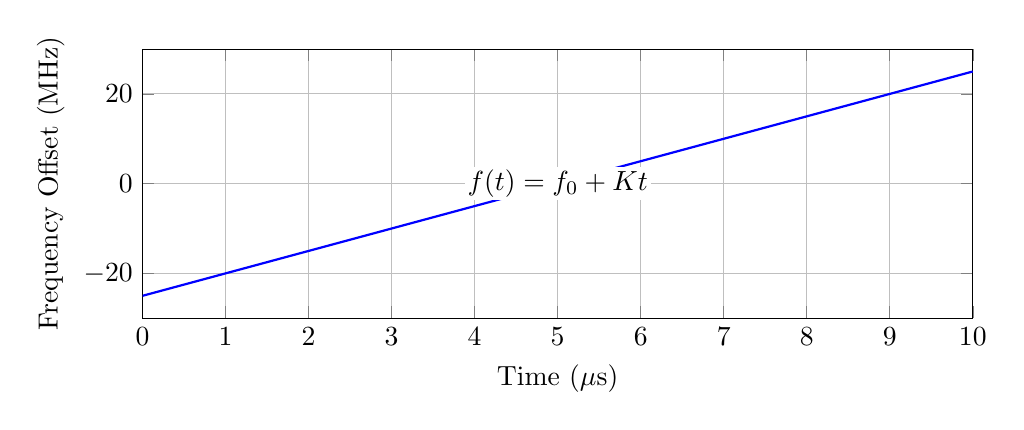
\begin{tikzpicture}
\begin{axis}[
    width=\textwidth, height=5cm,
    xlabel={Time ($\mu$s)},
    ylabel={Frequency Offset (MHz)},
    xmin=0, xmax=10,
    ymin=-30, ymax=30,
    grid=both,
]
    \addplot[thick, blue, domain=0:10] {-25 + 5*x};
    \node at (axis cs:5,0) [fill=white, inner sep=1pt] {$f(t) = f_0 + Kt$};
\end{axis}
\end{tikzpicture}
\caption{Instantaneous frequency vs time}
\end{subfigure}
\hfill
\begin{subfigure}[b]{0.48\textwidth}
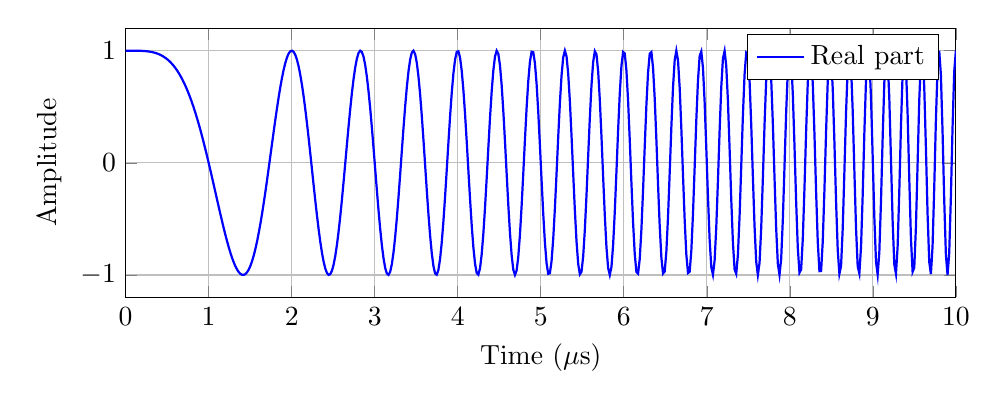
\begin{tikzpicture}
\begin{axis}[
    width=\textwidth, height=5cm,
    xlabel={Time ($\mu$s)},
    ylabel={Amplitude},
    xmin=0, xmax=10,
    ymin=-1.2, ymax=1.2,
    grid=both,
    ytick={-1,0,1},
]
    \addplot[thick, blue, domain=0:10, samples=500] {cos(deg(pi*0.5*x*x))};
    \addlegendentry{Real part}
\end{axis}
\end{tikzpicture}
\caption{Real part of chirp signal}
\end{subfigure}
\caption{LFM chirp waveform. Left: Frequency increases linearly from $-B/2$ to $+B/2$. Right: The resulting oscillation with increasing frequency.}
\label{fig:chirp}
\end{figure}

\subsection{Single Echo Generation}

For a ray hitting at range $R$:

\begin{figure}[htbp]
\centering
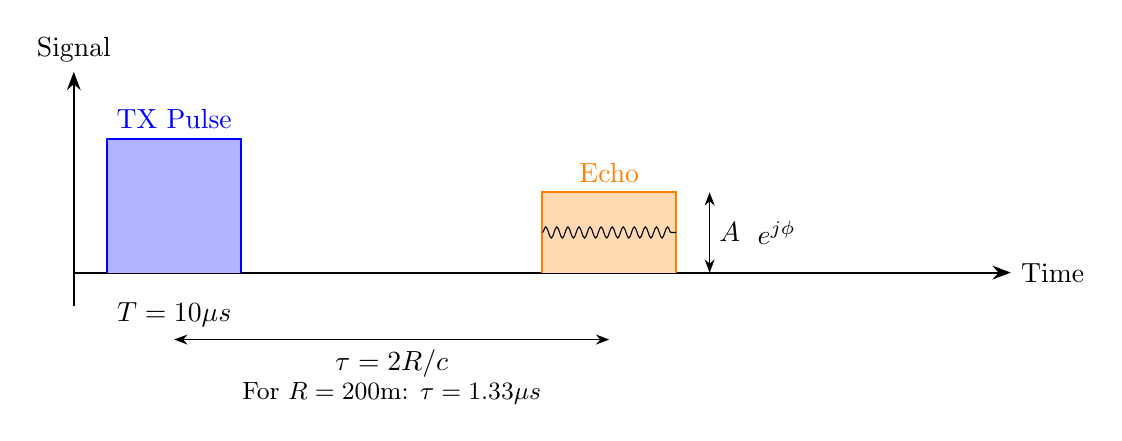
\begin{tikzpicture}[scale=0.85]
    % Timeline
    \draw[-{Stealth}, thick] (0,0) -- (14,0) node[right] {Time};
    \draw[-{Stealth}, thick] (0,-0.5) -- (0,3) node[above] {Signal};

    % TX pulse
    \fill[blue!30] (0.5,0) rectangle (2.5,2);
    \draw[thick, blue] (0.5,0) -- (0.5,2) -- (2.5,2) -- (2.5,0);
    \node[blue, above] at (1.5,2) {TX Pulse};
    \node[below] at (1.5,-0.3) {$T = 10\mu s$};

    % Echo (delayed)
    \fill[orange!30] (7,0) rectangle (9,1.2);
    \draw[thick, orange] (7,0) -- (7,1.2) -- (9,1.2) -- (9,0);
    \node[orange, above] at (8,1.2) {Echo};

    % Delay annotation
    \draw[{Stealth}-{Stealth}] (1.5,-1) -- (8,-1);
    \node[below] at (4.75,-1) {$\tau = 2R/c$};

    % Range example
    \node at (4.75,-1.8) {\small For $R=200$m: $\tau = 1.33\mu s$};

    % Amplitude annotation
    \draw[{Stealth}-{Stealth}] (9.5,0) -- (9.5,1.2);
    \node[right] at (9.5,0.6) {$A$};

    % Phase
    \draw[decorate, decoration={snake, amplitude=2pt, segment length=4pt}] (7,0.6) -- (9,0.6);
    \node at (10.5,0.6) {$e^{j\phi}$};

\end{tikzpicture}
\caption{Echo timing. The echo arrives after round-trip delay $\tau = 2R/c$ with amplitude $A$ and phase $\phi$.}
\label{fig:echo_timing}
\end{figure}

\subsubsection{Amplitude Calculation}

The echo amplitude includes multiple factors:

\begin{equation}
A = \underbrace{G_{2way}(\theta_{az}, \theta_{el})}_{\text{Antenna Pattern}} \cdot \underbrace{\frac{1}{R^2 + 1}}_{\text{Path Loss}} \cdot \underbrace{L_{atm}(R)}_{\text{Atmospheric}} \cdot \underbrace{|F|^2}_{\text{Multipath}}
\end{equation}

\paragraph{Antenna Pattern Weighting}

Each ray has an offset from boresight. The antenna gain at that offset determines how much power goes in that direction:

\begin{equation}
G_{2way} = \left[ \text{sinc}^2\left(\frac{2.783 \cdot \Delta\phi}{\theta_{az}}\right) \cdot \text{sinc}^2\left(\frac{2.783 \cdot \Delta\theta}{\theta_{el}}\right) \right]^2
\end{equation}

\paragraph{Atmospheric Attenuation}

At X-band, atmospheric gases absorb some energy:

\begin{equation}
L_{atm}(R) = 10^{-\gamma_{dB} \cdot 2R/(10 \cdot 1000)}
\end{equation}

where $\gamma_{dB} \approx 0.01$ dB/km combines oxygen and water vapor absorption.

\begin{figure}[htbp]
\centering
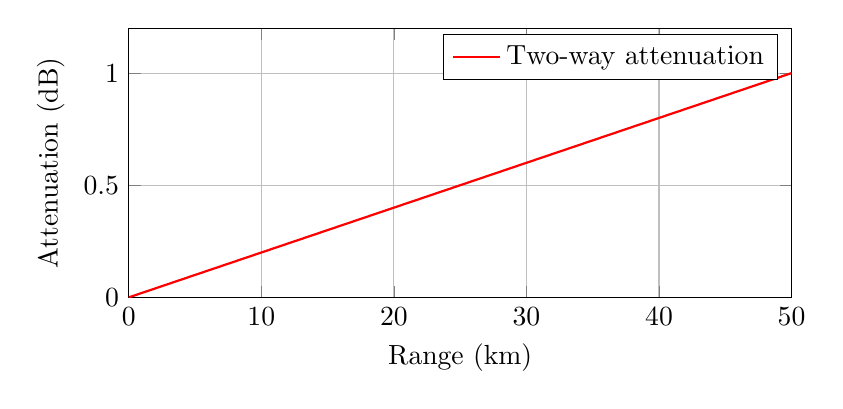
\begin{tikzpicture}
\begin{axis}[
    width=10cm, height=5cm,
    xlabel={Range (km)},
    ylabel={Attenuation (dB)},
    xmin=0, xmax=50,
    ymin=0, ymax=1.2,
    grid=both,
]
    \addplot[thick, red, domain=0:50] {0.01 * 2 * x};
    \addlegendentry{Two-way attenuation}
\end{axis}
\end{tikzpicture}
\caption{Atmospheric attenuation vs range at X-band. At 50 km, two-way loss is about 1 dB.}
\label{fig:atm_atten}
\end{figure}

\subsubsection{Phase Calculation}

The phase accumulates over the round-trip path:

\begin{equation}
\phi = \frac{4\pi f_0 R}{c} = \frac{4\pi R}{\lambda}
\end{equation}

\textbf{Key insight:} A range change of $\lambda/2 = 1.6$ cm causes a phase shift of $2\pi$ (360°).

\begin{figure}[htbp]
\centering
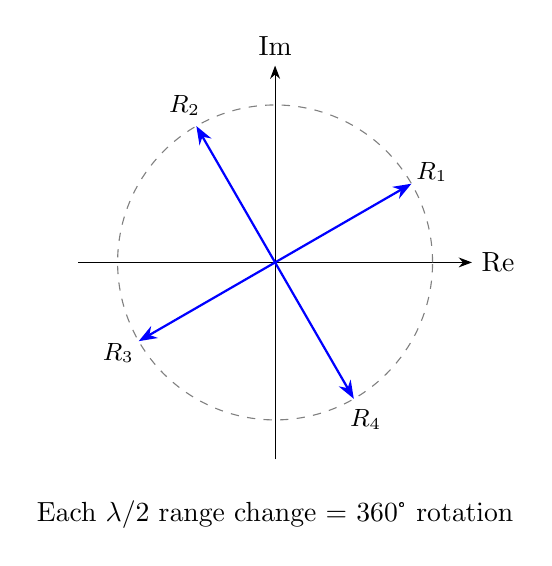
\begin{tikzpicture}
    % Phasor diagram
    \draw[-{Stealth}] (-2.5,0) -- (2.5,0) node[right] {Re};
    \draw[-{Stealth}] (0,-2.5) -- (0,2.5) node[above] {Im};

    % Unit circle
    \draw[gray, dashed] (0,0) circle (2);

    % Multiple phasors at different ranges
    \foreach \angle/\label in {30/R_1, 120/R_2, 210/R_3, 300/R_4} {
        \draw[-{Stealth}, thick, blue] (0,0) -- ({2*cos(\angle)},{2*sin(\angle)});
        \node at ({2.3*cos(\angle)},{2.3*sin(\angle)}) {\small $\label$};
    }

    \node at (0,-3.2) {Each $\lambda/2$ range change = 360° rotation};
\end{tikzpicture}
\caption{Phasor representation of echoes at different ranges. The phase rotates rapidly with range due to the short wavelength.}
\label{fig:phasor}
\end{figure}

\subsection{Multipath: Two-Ray Model}

When a target is above a reflective surface, two paths exist:

\begin{figure}[htbp]
\centering
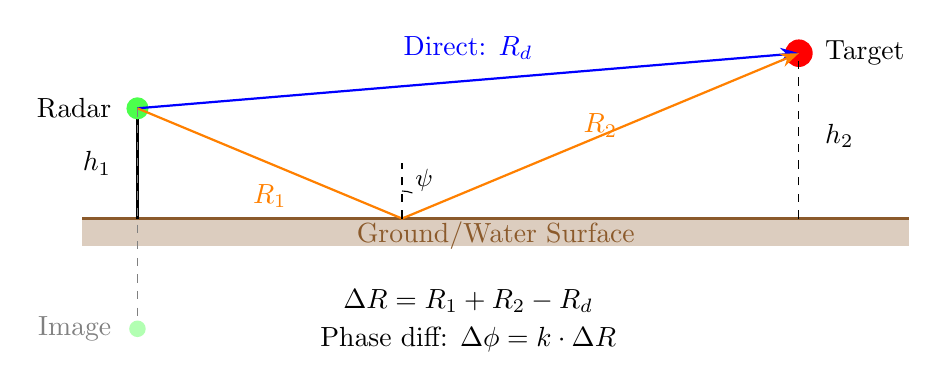
\begin{tikzpicture}[scale=0.7]
    % Ground
    \fill[groundcolor!30] (-1,-0.5) rectangle (14,0);
    \draw[thick, groundcolor] (-1,0) -- (14,0);
    \node[groundcolor] at (6.5,-0.3) {Ground/Water Surface};

    % Radar
    \draw[thick] (0,0) -- (0,2);
    \fill[green!70] (0,2) circle (0.2);
    \node[left] at (-0.3,2) {Radar};
    \node[left] at (-0.3,1) {$h_1$};

    % Target
    \fill[red] (12,3) circle (0.25);
    \node[right] at (12.3,3) {Target};
    \node[right] at (12.3,1.5) {$h_2$};
    \draw[dashed] (12,0) -- (12,3);

    % Direct path
    \draw[thick, blue, -{Stealth}] (0,2) -- (12,3);
    \node[blue, above, sloped] at (6,2.7) {Direct: $R_d$};

    % Reflected path
    \coordinate (reflect) at (4.8,0);
    \draw[thick, orange] (0,2) -- (reflect);
    \draw[thick, orange, -{Stealth}] (reflect) -- (12,3);
    \node[orange, below, sloped] at (2.4,0.8) {$R_1$};
    \node[orange, above, sloped] at (8.4,1.3) {$R_2$};

    % Reflection angle
    \draw[dashed] (reflect) -- ++(0,1);
    \draw ($(reflect)+(0,0.5)$) arc (90:68:0.5);
    \node at ($(reflect)+(0.4,0.7)$) {\small $\psi$};

    % Image
    \draw[dashed, gray] (0,2) -- (0,-2);
    \fill[green!30] (0,-2) circle (0.15);
    \node[gray, left] at (-0.3,-2) {Image};

    % Path difference annotation
    \node at (6,-1.5) {$\Delta R = R_1 + R_2 - R_d$};
    \node at (6,-2.2) {Phase diff: $\Delta\phi = k \cdot \Delta R$};

\end{tikzpicture}
\caption{Two-ray multipath geometry. The direct path interferes with the ground-reflected path, causing constructive or destructive interference depending on path difference.}
\label{fig:multipath}
\end{figure}

The multipath propagation factor is:

\begin{equation}
F = 1 + \Gamma \cdot \rho_s \cdot D \cdot e^{-jk\Delta R} \cdot \frac{R_d}{R_1 + R_2}
\end{equation}

where:
\begin{itemize}
    \item $\Gamma$ = Fresnel reflection coefficient (complex, depends on polarization)
    \item $\rho_s$ = Roughness factor (reduces specular reflection)
    \item $D$ = Divergence factor (spherical Earth effect)
    \item $k = 2\pi/\lambda$ = Wavenumber
\end{itemize}

\subsection{Complete Echo Signal}

For hit $i$ at range $R_i$:

\begin{equation}
\text{echo}_i(t) = A_i \cdot e^{j\phi_i} \cdot s_{TX}(t)
\end{equation}

Added to received signal at the correct delay:

\begin{equation}
s_{RX}(t) = \sum_{i=1}^{N_{hits}} \text{echo}_i\left(t - \frac{2R_i}{c}\right)
\end{equation}

%=============================================================================
\section{Stage 5: Pulse Compression}
%=============================================================================

\subsection{The Matched Filter}

Pulse compression correlates the received signal with the transmitted waveform:

\begin{equation}
s_{compressed}(t) = s_{RX}(t) \star s_{TX}^*(-t) = \mathcal{F}^{-1}\left\{ S_{RX}(f) \cdot S_{TX}^*(f) \right\}
\end{equation}

\begin{figure}[htbp]
\centering
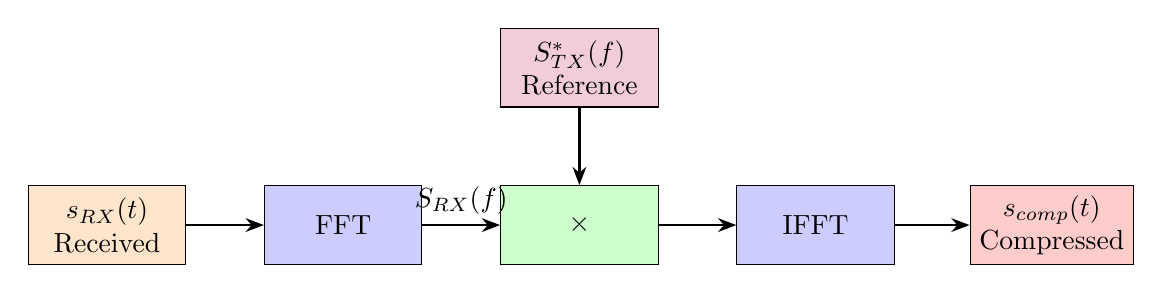
\begin{tikzpicture}[
    box/.style={rectangle, draw, minimum width=2cm, minimum height=1cm, align=center},
    arrow/.style={-{Stealth}, thick}
]
    % Input signal
    \node[box, fill=orange!20] (rx) at (0,0) {$s_{RX}(t)$\\Received};

    % FFT
    \node[box, fill=blue!20] (fft1) at (3,0) {FFT};

    % Multiply
    \node[box, fill=green!20] (mult) at (6,0) {$\times$};

    % Reference
    \node[box, fill=purple!20] (ref) at (6,2) {$S_{TX}^*(f)$\\Reference};

    % IFFT
    \node[box, fill=blue!20] (ifft) at (9,0) {IFFT};

    % Output
    \node[box, fill=red!20] (out) at (12,0) {$s_{comp}(t)$\\Compressed};

    % Arrows
    \draw[arrow] (rx) -- (fft1);
    \draw[arrow] (fft1) -- (mult) node[midway, above] {$S_{RX}(f)$};
    \draw[arrow] (ref) -- (mult);
    \draw[arrow] (mult) -- (ifft);
    \draw[arrow] (ifft) -- (out);

\end{tikzpicture}
\caption{FFT-based matched filter implementation. Correlation in time domain equals multiplication in frequency domain.}
\label{fig:matched_filter}
\end{figure}

\subsection{Compression Result}

The matched filter output for an LFM chirp is a sinc function:

\begin{equation}
|s_{compressed}(\tau)| \propto \left| \text{sinc}(B \cdot \tau) \right|
\end{equation}

\begin{figure}[htbp]
\centering
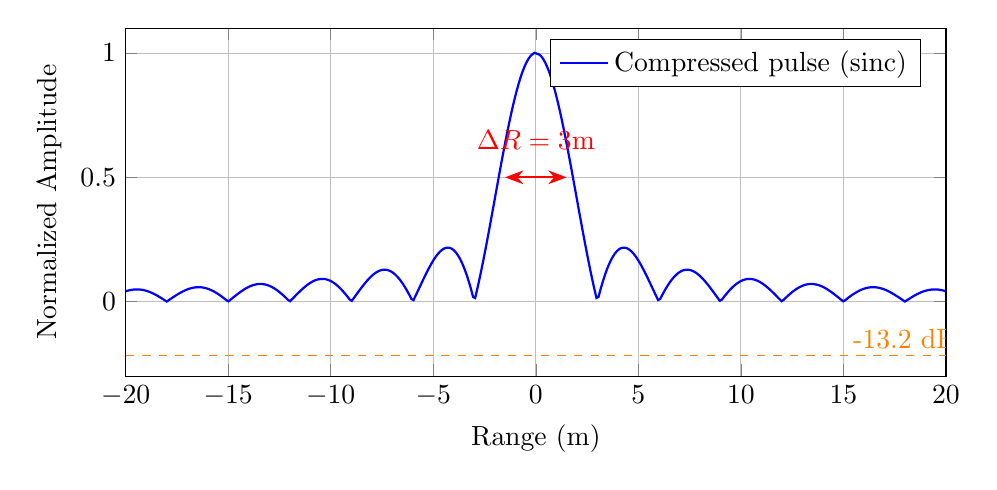
\begin{tikzpicture}
\begin{axis}[
    width=12cm, height=6cm,
    xlabel={Range (m)},
    ylabel={Normalized Amplitude},
    xmin=-20, xmax=20,
    ymin=-0.3, ymax=1.1,
    grid=both,
    legend pos=north east
]
    % Sinc function
    \addplot[thick, blue, domain=-20:20, samples=400] {
        abs(sin(deg(pi*x/3))/(pi*x/3 + 0.0001))
    };
    \addlegendentry{Compressed pulse (sinc)}

    % Main lobe width
    \draw[{Stealth}-{Stealth}, thick, red] (axis cs:-1.5,0.5) -- (axis cs:1.5,0.5);
    \node[red] at (axis cs:0,0.65) {$\Delta R = 3$m};

    % Sidelobe level
    \draw[dashed, orange] (axis cs:-20,-0.217) -- (axis cs:20,-0.217);
    \node[orange, right] at (axis cs:15,-0.15) {-13.2 dB};

\end{axis}
\end{tikzpicture}
\caption{Matched filter output showing sinc function. Main lobe width equals range resolution. First sidelobe at -13.2 dB without windowing.}
\label{fig:compressed_pulse}
\end{figure}

\subsection{Windowing for Sidelobe Reduction}

Applying a Hamming window to the reference waveform reduces sidelobes at the cost of slightly wider main lobe:

\begin{equation}
w(n) = 0.54 - 0.46 \cos\left(\frac{2\pi n}{N-1}\right)
\end{equation}

\begin{figure}[htbp]
\centering
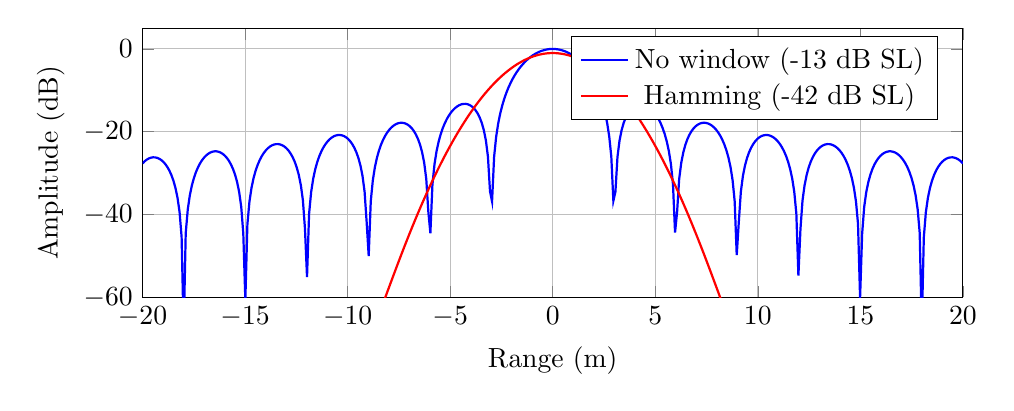
\begin{tikzpicture}
\begin{axis}[
    width=12cm, height=5cm,
    xlabel={Range (m)},
    ylabel={Amplitude (dB)},
    xmin=-20, xmax=20,
    ymin=-60, ymax=5,
    grid=both,
    legend pos=north east
]
    % Unwindowed (sinc)
    \addplot[thick, blue, domain=-20:20, samples=400] {
        20*log10(abs(sin(deg(pi*x/3))/(pi*x/3 + 0.0001)) + 0.0001)
    };
    \addlegendentry{No window (-13 dB SL)}

    % Windowed (approximation)
    \addplot[thick, red, domain=-20:20, samples=400] {
        20*log10(exp(-0.5*(x/2.2)^2) + 0.0001) - 1
    };
    \addlegendentry{Hamming (-42 dB SL)}

\end{axis}
\end{tikzpicture}
\caption{Effect of windowing on pulse compression. Hamming window reduces sidelobes from -13 dB to -42 dB.}
\label{fig:windowing}
\end{figure}

%=============================================================================
\section{Stage 6: PPI Processing}
%=============================================================================

After running the simulation for all 720 azimuths, we have a raw PPI:

\begin{equation}
\text{PPI}_{raw}[\phi, R] = |s_{compressed}|^2, \quad \phi \in [0°, 359.5°], \quad R \in [0, R_{max}]
\end{equation}

This shows \textbf{ray artifacts}---targets appear as thin radial lines because each ray deposits energy in only one azimuth bin.

\subsection{Beam Spreading (Azimuth Convolution)}

Real targets are illuminated for the entire time the beam sweeps past them. We simulate this by convolving along azimuth:

\begin{equation}
\text{PPI}_{spread}[\phi, R] = \text{PPI}_{raw}[\phi, R] \star_\phi g(\phi)
\end{equation}

where $g(\phi)$ is a Gaussian kernel with $\sigma = \theta_{3dB}/2.355$:

\begin{figure}[htbp]
\centering
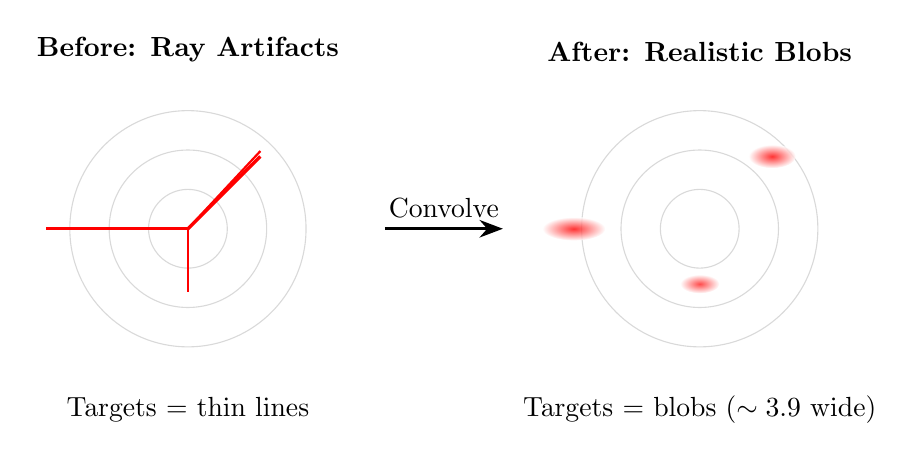
\begin{tikzpicture}
    % Before
    \begin{scope}[shift={(0,0)}]
        \node[above] at (2,4) {\textbf{Before: Ray Artifacts}};

        % Polar grid
        \draw[gray!30] (2,2) circle (1.5);
        \draw[gray!30] (2,2) circle (1);
        \draw[gray!30] (2,2) circle (0.5);

        % Thin radial lines (artifacts)
        \draw[red, very thick] (2,2) -- ++(45:1.3);
        \draw[red, thick] (2,2) -- ++(47:1.35);
        \draw[red, very thick] (2,2) -- ++(180:1.8);
        \draw[red, thick] (2,2) -- ++(270:0.8);

        \node at (2,-0.3) {Targets = thin lines};
    \end{scope}

    % Arrow
    \draw[-{Stealth}, very thick] (4.5,2) -- (6,2) node[midway, above] {Convolve};

    % After
    \begin{scope}[shift={(6.5,0)}]
        \node[above] at (2,4) {\textbf{After: Realistic Blobs}};

        % Polar grid
        \draw[gray!30] (2,2) circle (1.5);
        \draw[gray!30] (2,2) circle (1);
        \draw[gray!30] (2,2) circle (0.5);

        % Spread blobs
        \shade[inner color=red, outer color=white, opacity=0.8] ($(2,2)+(45:1.3)$) ellipse (0.3 and 0.15);
        \shade[inner color=red, outer color=white, opacity=0.8] ($(2,2)+(180:1.6)$) ellipse (0.4 and 0.15);
        \shade[inner color=red, outer color=white, opacity=0.7] ($(2,2)+(270:0.7)$) ellipse (0.25 and 0.12);

        \node at (2,-0.3) {Targets = blobs ($\sim 3.9°$ wide)};
    \end{scope}
\end{tikzpicture}
\caption{Effect of beam spreading convolution. Thin radial artifacts become realistic blob-shaped returns matching the antenna beamwidth.}
\label{fig:beam_spreading}
\end{figure}

\subsection{2D Point Spread Function}

A complete radar PSF spreads energy in both range and azimuth:

\begin{equation}
\text{PSF}(R, \phi) = \underbrace{\text{sinc}^2\left(\frac{R}{\Delta R}\right)}_{\text{Range (matched filter)}} \cdot \underbrace{\exp\left(-\frac{\phi^2}{2\sigma_\phi^2}\right)}_{\text{Azimuth (antenna)}}
\end{equation}

\begin{figure}[htbp]
\centering
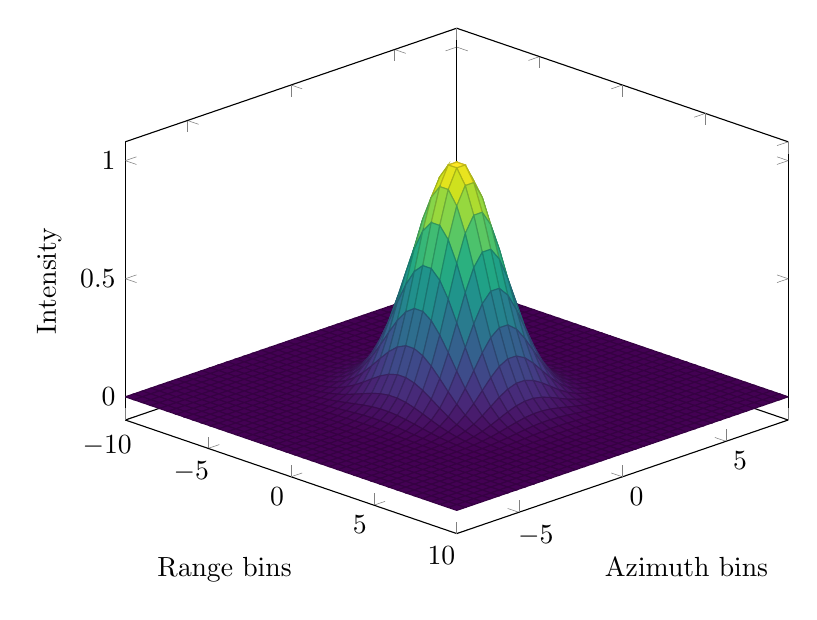
\begin{tikzpicture}
\begin{axis}[
    view={45}{30},
    width=10cm, height=8cm,
    xlabel={Range bins},
    ylabel={Azimuth bins},
    zlabel={Intensity},
    colormap/viridis,
]
    \addplot3[
        surf,
        domain=-10:10,
        domain y=-8:8,
        samples=40,
    ] {exp(-x^2/8 - y^2/4)};
\end{axis}
\end{tikzpicture}
\caption{2D radar Point Spread Function. The PSF is narrower in range (from pulse compression) and wider in azimuth (from beamwidth).}
\label{fig:psf2d}
\end{figure}

\subsection{Polar to Cartesian Conversion}

Finally, we convert from radar coordinates $(R, \phi)$ to image coordinates $(x, y)$:

\begin{align}
x &= R \sin(\phi) \\
y &= R \cos(\phi)
\end{align}

\begin{figure}[htbp]
\centering
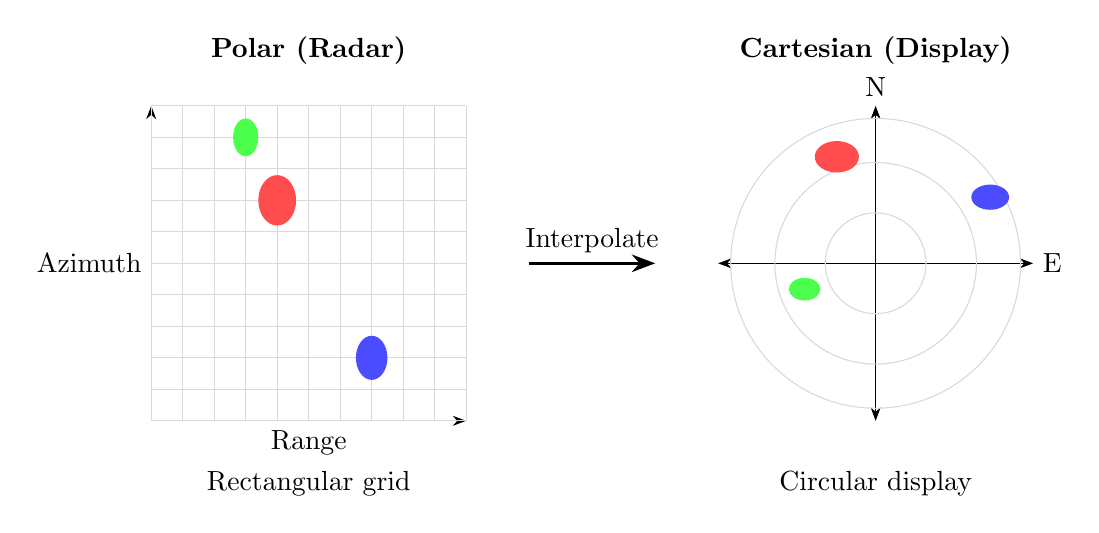
\begin{tikzpicture}[scale=0.8]
    % Polar representation
    \begin{scope}[shift={(0,0)}]
        \node[above] at (2.5,5.5) {\textbf{Polar (Radar)}};

        \draw[{Stealth}-{Stealth}] (0,5) -- (0,0) -- (5,0);
        \node[below] at (2.5,0) {Range};
        \node[left] at (0,2.5) {Azimuth};

        % Grid
        \draw[gray!30, step=0.5] (0,0) grid (5,5);

        % Target blobs in polar
        \fill[red!70] (2,3.5) ellipse (0.3 and 0.4);
        \fill[blue!70] (3.5,1) ellipse (0.25 and 0.35);
        \fill[green!70] (1.5,4.5) ellipse (0.2 and 0.3);

        \node at (2.5,-1) {Rectangular grid};
    \end{scope}

    % Arrow
    \draw[-{Stealth}, very thick] (6,2.5) -- (8,2.5) node[midway, above] {Interpolate};

    % Cartesian representation
    \begin{scope}[shift={(9,0)}]
        \node[above] at (2.5,5.5) {\textbf{Cartesian (Display)}};

        \draw[{Stealth}-{Stealth}] (0,2.5) -- (5,2.5);
        \draw[{Stealth}-{Stealth}] (2.5,0) -- (2.5,5);
        \node[right] at (5,2.5) {E};
        \node[above] at (2.5,5) {N};

        % Range rings
        \draw[gray!30] (2.5,2.5) circle (0.8);
        \draw[gray!30] (2.5,2.5) circle (1.6);
        \draw[gray!30] (2.5,2.5) circle (2.3);

        % Target blobs in Cartesian (transformed)
        \fill[red!70] ($(2.5,2.5)+(110:1.8)$) ellipse (0.35 and 0.25);
        \fill[blue!70] ($(2.5,2.5)+(30:2.1)$) ellipse (0.3 and 0.2);
        \fill[green!70] ($(2.5,2.5)+(200:1.2)$) ellipse (0.25 and 0.18);

        \node at (2.5,-1) {Circular display};
    \end{scope}
\end{tikzpicture}
\caption{Polar to Cartesian scan conversion. Bilinear interpolation fills gaps in the Cartesian grid.}
\label{fig:scan_conversion}
\end{figure}

%=============================================================================
\section{Complete Signal Flow Example}
%=============================================================================

Let's trace a single target through the entire simulation:

\begin{figure}[htbp]
\centering
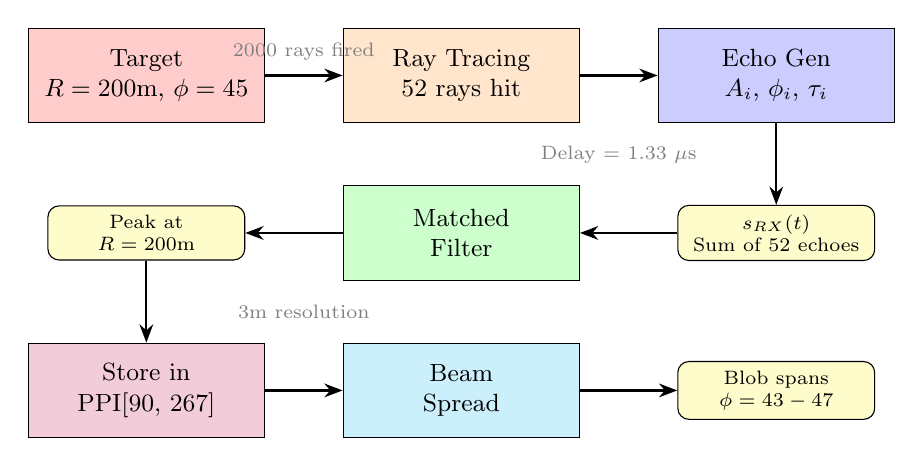
\begin{tikzpicture}[
    box/.style={rectangle, draw, minimum width=3cm, minimum height=1.2cm, align=center, font=\small},
    data/.style={rectangle, rounded corners, draw, fill=yellow!20, minimum width=2.5cm, align=center, font=\scriptsize},
    arrow/.style={-{Stealth}, thick}
]
    % Target info
    \node[box, fill=red!20] (target) at (0,0) {Target\\$R = 200$m, $\phi = 45°$};

    % Ray hits
    \node[box, fill=orange!20] (hits) at (4,0) {Ray Tracing\\52 rays hit};

    % Echo generation
    \node[box, fill=blue!20] (echo) at (8,0) {Echo Gen\\$A_i$, $\phi_i$, $\tau_i$};

    % Received signal
    \node[data] (rx) at (8,-2) {$s_{RX}(t)$\\Sum of 52 echoes};

    % Matched filter
    \node[box, fill=green!20] (mf) at (4,-2) {Matched\\Filter};

    % Compressed
    \node[data] (comp) at (0,-2) {Peak at\\$R = 200$m};

    % Store in PPI
    \node[box, fill=purple!20] (ppi) at (0,-4) {Store in\\PPI[90, 267]};

    % Beam spread
    \node[box, fill=cyan!20] (spread) at (4,-4) {Beam\\Spread};

    % Final
    \node[data] (final) at (8,-4) {Blob spans\\$\phi = 43° - 47°$};

    % Arrows
    \draw[arrow] (target) -- (hits);
    \draw[arrow] (hits) -- (echo);
    \draw[arrow] (echo) -- (rx);
    \draw[arrow] (rx) -- (mf);
    \draw[arrow] (mf) -- (comp);
    \draw[arrow] (comp) -- (ppi);
    \draw[arrow] (ppi) -- (spread);
    \draw[arrow] (spread) -- (final);

    % Annotations
    \node[gray, font=\scriptsize] at (2,0.3) {2000 rays fired};
    \node[gray, font=\scriptsize] at (6,-1) {Delay = 1.33 $\mu$s};
    \node[gray, font=\scriptsize] at (2,-3) {3m resolution};

\end{tikzpicture}
\caption{Complete signal flow for a single target at 200m range, 45° azimuth.}
\label{fig:signal_flow}
\end{figure}

\subsection{Numerical Example}

For a target at $R = 200$ m, $\phi = 45°$:

\begin{enumerate}
    \item \textbf{Delay:} $\tau = 2R/c = 2 \times 200 / (3 \times 10^8) = 1.33$ $\mu$s $= 267$ samples at 200 MSPS

    \item \textbf{Phase:} $\phi = 4\pi f_0 R / c = 4\pi \times 9.41 \times 10^9 \times 200 / (3 \times 10^8) = 78,873$ rad $= 12,553$ cycles

    \item \textbf{Antenna Gain:} If ray is 1° off boresight: $G = \text{sinc}^2(2.783 \times 1° / 3.9°) = 0.67$ (one-way)

    \item \textbf{Two-way:} $G_{2way} = 0.67^4 = 0.20$ (-7 dB)

    \item \textbf{Range Bin:} After compression, peak appears at bin $267 \times 0.75$m $\approx 200$m

    \item \textbf{Azimuth Bin:} $45° / 0.5° = 90$th bin
\end{enumerate}

%=============================================================================
\section{Summary}
%=============================================================================

\begin{table}[htbp]
\centering
\begin{tabular}{lp{8cm}}
\toprule
\textbf{Stage} & \textbf{Key Physics} \\
\midrule
3D World & Triangle meshes, Möller-Trumbore intersection \\
Ray Tracing & Monte Carlo sampling within antenna beam \\
Echo Generation & $A \cdot e^{j\phi} \cdot s_{TX}$, includes path loss, multipath, atmosphere \\
Pulse Compression & FFT correlation, sinc response, windowing for sidelobes \\
Beam Spreading & Gaussian convolution matching beamwidth \\
PSF & 2D spreading in range and azimuth \\
Scan Conversion & Bilinear interpolation, polar to Cartesian \\
\bottomrule
\end{tabular}
\caption{Summary of physics at each simulation stage}
\end{table}

\end{document}
